\section{Reti di calcolatori e Internet}

\subsection{Cos'è internet?}
\textbf{Internet} è una rete globale di calcolatori interconnessi, spesso descritta come una 'rete di reti', che comunica utilizzando un insieme comune di protocolli, principalmente la suite TCP/IP.
\subsubsection{Definizioni varie}
\begin{description}[font=\sffamily\bfseries, leftmargin=1cm, style=nextline]
  \item[host] 
    o \textit{sistemi periferici} sistema terminale della rete dove risiedono e vengono eseguite le applicazioni.
  \item[rete di collegamenti]
    o \textit{communication link} il mezzo fisico (es. cavo coassiale, fibra ottica, onde radio) attraverso cui i dati vengono trasmessi tra i nodi della rete.
  \item[commutatori di pacchetti]
    o \textit{packet switch} dispositivi di rete che inoltrano i pacchetti di dati da un collegamento in ingresso a un collegamento in uscita.
  \item[velocità di trasmissione]
    o \textit{transimission rate} velocità con cui i vari tipi di collegamenti si scambiano dati, misurata in \textbf{bit/secondo (bps)} e che rappresenta la capacità del collegamento..
  \item[pacchetto]
    o \textit{packet} unità di dati formata a livello di rete (livello IP), contenente una porzione di dati (che a livello di trasporto, con TCP, è chiamata \textbf{segmento}) e un'intestazione con informazioni di controllo. 
  \item[commutatore di pacchetto]
    dispositivo che riceve un \textbf{pacchetto} su un collegamento in ingresso, lo memorizza temporaneamente e poi lo ritrasmette su un collegamento in uscita. I due tipi principali sono i \textbf{router}, usati nel nucleo della rete per l'instradamento tra reti diverse, e i \textbf{commutatori a livello di collegamento \textit{(link-layer switch)}}, usati nelle reti locali per la commutazione all'interno della stessa rete. 
  \item[percorso]
    o \textit{route} o \textit{path}, sequenza di collegamenti e di commutatori di pacchetto attraversata dal singolo pacchetto. 
  \item[Internet ServiceProvider (ISP)]
    un'organizzazione che possiede e gestisce un insieme di commutatori di pacchetto e di collegamenti, fornendo ai sistemi periferici e ad altre reti l'accesso a Internet.
  \item[applicazioni distribuite]
    o \textit{distributed applications}, più sistemi periferici che si scambiano reciprocamente dati. Vengono eseguite sui sistemi periferici (\textit{host}).
  \item[interfaccia socket]
    o \textit{socket interface} un'interfaccia di programmazione (API) che specifica come un programma eseguito su un sistema periferico può richiedere ai servizi di rete di Internet di recapitare dati a un programma eseguito su un altro sistema periferico.
  \item[protocollo]
    è un insieme di regole rigido, definisce il formato, l’ordine dei messaggi scambiati tra due o più entità in comunicazione, così come le azioni intraprese in fase di trasmissione e/o di ricezione di un messaggio o di un altro evento.
  \item[client e server]
    \textit{host} che richiedono dei servizi (client) e \textit{host} che si occupano di erogare dei servizi (server). Questi ultimi sono spesso collocati in potenti \textbf{data center} per garantire alta disponibilità e prestazioni. 
  \item[reti di accesso]
    o \textit{access network} la rete che connette fisicamente i sistemi periferici al primo \textbf{router} (chiamato \textbf{router di bordo}, o \textit{edge router}) sul percorso verso la rete Internet del provider. 
\end{description}

\subsection{Il nucleo della rete}
Il nucleo della rete è una maglia complessa di commutatori di pacchetti e collegamenti ad alta velocità che interconnettono i sistemi periferici di Internet. La funzione principale del nucleo della rete è quella di instradare i dati tra i sistemi periferici.

\subsubsection{Commutazione di pacchetto}
Le \textit{applicazioni distribuite} scambiano \textbf{messaggi}. Per facilitare la trasmissione e la gestione della rete, la sorgente divide i messaggi più lunghi in unità più piccole chiamate \textit{pacchetti}, che viaggiano attraverso i \textit{commutatori di pacchetto} per raggiungere la destinazione. Ogni pacchetto viene trasmesso sul collegamento fisico alla velocità di trasmissione $R$ (misurata in bit al secondo, bps). Un pacchetto di $L$ bit impiegherà quindi $L/R$ secondi per essere trasmesso completamente sul collegamento.

Una delle tecnologie fondamentali utilizzate dai \textit{commutatori di pacchetto} è la \textbf{trasmissione store and forward}. Secondo questo principio, il commutatore deve ricevere *completamente* l'intero \textit{pacchetto} prima di iniziare a trasmettere il primo bit verso il collegamento di uscita.

Consideriamo un pacchetto di $L$ bit che viene trasmesso dall'\textit{host} sorgente al primo \textit{router} sul percorso. Se la velocità di trasmissione del collegamento è $R$, il tempo necessario per trasmettere il pacchetto è $L/R$ secondi. Utilizzando la trasmissione store and forward, il router riceverà l'intero pacchetto all'istante $L/R$. Supponendo che anche il collegamento tra il router e l'\textit{host} di destinazione abbia una velocità di trasmissione $R$, il router inizierà a trasmettere il pacchetto verso la destinazione. L'\textit{host} di destinazione riceverà l'intero pacchetto all'istante $L/R$ (trasmissione host-router) + $L/R$ (trasmissione router-host) = $2L/R$.

Generalizzando, considerando un percorso con $N$ collegamenti, ognuno con una velocità di trasmissione $R$, e quindi $N-1$ router intermedi che utilizzano la trasmissione store and forward, il ritardo totale di trasmissione attraverso il percorso (trascurando altri tipi di ritardi come la propagazione) sarà:
\[
  delay = N \frac{L}{R}
\]

Se la sorgente deve inviare $P$ pacchetti in sequenza sullo stesso percorso, il tempo necessario affinché l'ultimo pacchetto raggiunga la destinazione sarà approssimativamente $P \cdot N \frac{L}{R}$, assumendo che ogni pacchetto venga trasmesso solo dopo che il precedente è stato completamente trasmesso.

\textit{Nota:} Se i pacchetti vengono inviati in modo continuo (\textit{pipelining}), l'analisi del ritardo diventa più complessa. Il ritardo per il primo pacchetto rimane $N \frac{L}{R}$, ma i pacchetti successivi arriveranno a intervalli di $\frac{L}{R}$.

Trascurando però i ritardi di propagazione, che rappresentano il tempo impiegato dal segnale per viaggiare attraverso il mezzo fisico.

I commutatori di pacchetto hanno più collegamenti, e per ogni collegamento di output è presente un \textbf{buffer di output} o \textbf{coda di output} per organizzare i pacchetti da inviare su quel collegamento. Questo comporta che i pacchetti subiscono un \textbf{ritardo di accodamento}, il pacchetto deve aspettare che si "liberi il passaggio" per essere trasmesso. Questo ritardo è variabile e dipende dal traffico della rete in un dato momento. Nel caso in cui il buffer sia pieno, avendo una dimensione prestabilita, il pacchetto verrà perso (\textit{packet loss}), verrà eliminato o il pacchetto in arrivo o uno di quelli in coda, dipende dal progettista di rete.

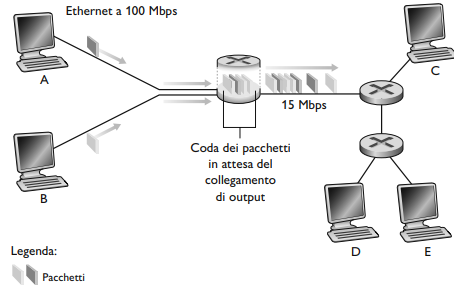
\includegraphics[width=\textwidth, height=6cm, keepaspectratio]{img/commutazione_di_pacchetto.png}

\subsubsection{Commutazione di circuito}
Esiste un altro metodo per scambiare messaggi, ossia la \textbf{commutazione di circuito}. Questo garantisce che le risorse per consentire lo scambio di dati sono \textbf{dedicate} (o \textbf{riservate}), sono quindi esclusivamente allocate per la \textbf{comunicazione}.

Bisogna stabilire un collegamento tra mittente e destinatario, lo chiameremo \textbf{circuito}, attraverso una fase di segnalazione tra i commutatori. A questo circuito verrà riservata una \textbf{velocità di trasmissione costante} (pari a una frazione della capacità del canale).

Ogni \textit{host} della rete è connesso a un commutatore che a sua volta è connesso con gli altri \textit{host} nella rete. Quando un host dovrà comunicare con un altro host, verrà instaurata una \textbf{connessione punto a punto} (\textit{connessione end to end}) *logica* a loro dedicata.

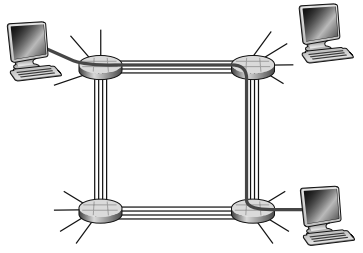
\includegraphics[width=\textwidth, height=6cm, keepaspectratio]{img/commutazione_di_circuito.png}

Un circuito viene implementato tramite \textbf{multiplexing a divisione di frequenza} (\textit{frequency-division multiplexing}) o \textbf{multiplexing a divisione di tempo} (\textit{time-division multiplexing}).

Con il \textbf{FDM} (multiplexing a divisione di frequenza), lo spettro di frequenza disponibile viene diviso in bande di frequenza più piccole, ognuna delle quali viene dedicata a una connessione. A ciascuna connessione viene quindi dedicata un'\textbf{ampiezza di banda} (\textit{bandwidth}) specifica.

Con il \textbf{TDM} (multiplexing a divisione di tempo), il tempo viene diviso in intervalli (slot di tempo) e a ciascuna connessione viene assegnato uno slot di tempo in cui può trasmettere i dati. Gli slot di tempo vengono assegnati in modo ciclico.

\subsection{Ritardi, perdite e throughput nelle reti a commutazione di pacchetto}
Per le leggi fisiche non è possibile scambiare dati istantaneamente. Le reti introducono ritardi, perdono pacchetti e limitano il \textbf{throughput} (la quantità di dati al secondo che può essere trasferita tra due sistemi periferici) a causa di fattori come la congestione della rete e le limitazioni fisiche dei collegamenti.

Esistono modi per affrontare questo problema. 

\subsubsection{Panoramica del ritardo nelle reti a commutazione di pacchetto}
I principali tipi di ritardi sono:
\begin{itemize}
  \item \textbf{ritardo di elaborazione} (\textit{processing delay}): include il tempo per esaminare l'intestazione del pacchetto e determinare dove trasmetterlo e il tempo per controllare se ci sono errori a livello di bit.  
  \item \textbf{ritardo di accodamento} (\textit{queuing delay}): il pacchetto in coda attende la trasmissione sul collegamento nel caso in cui il buffer non sia libero. Questo ritardo è variabile e dipende dalla congestione della rete. Nel caso in cui il buffer sia libero, il ritardo è nullo.
  \item \textbf{ritardo di trasmissione} (\textit{trasmission delay}): utilizzando la politica \textbf{FIFO}. Avendo $L$ bit da trasmettere con $R$ bps di velocità di trasmissione, avremmo un ritardo pari a $L/R$, cioè il tempo richiesto per la tramissione di tutti i bit nel collegamento. 
  \item \textbf{ritardo di propagazione} (\textit{propagation delay}): tempo che il pacchetto impiega una volta immesso sul collegamento, viaggia a una velocità di propagazione del collegamento $v$ per una distanza $d$, quindi il ritardo sarà $d/v$.  
\end{itemize}
che sommati formano il \textbf{ritardo totale di nodo} (\textit{node delay}), ovvero la somma del ritardo di elaborazione, accodamento, trasmissione e propagazione:
\[
  d_{nodo} = d_{elaborazione} + d_{accodamento} + d_{trasmissione} + d_{propagazione} 
\]

\subsubsection{Ritardo end-to-end} 
\subsubsection{Throughput nelle reti di calcolatori} 

\subsection{Livelli dei protocolli e loro modelli di servizio - importante} 
\subsubsection{Architettura a livelli}
\subsubsection{Incapsulamento}

